\textit{Pour chacune des affirmations suivantes, indiquer si elle est vraie ou fausse.\\Chaque réponse doit être justifiée. Une réponse non justifiée ne rapporte aucun point.}

\smallskip

\begin{enumerate}
	\item On considère la fonction $f$ définie $\R$ par $f(x)=\e^x+x$.
	
	\textbf{Affirmation A} : La fonction $f$ admet pour tableau de variations le tableau ci-dessous :
	
	\begin{Centrage}
		\begin{tikzpicture}
			\tkzTabInit[lgt=3,espcl=6]{$x$/0.8,variations de $f$/1.6}{$-\infty$,$+\infty$}
			\tkzTabVar{-/$-\infty$,+/$+\infty$}
		\end{tikzpicture}
	\end{Centrage}
	
	\textbf{Affirmation B} : L’équation $f(x)=-2$ admet deux solutions dans $\R$.
	\item \textbf{Affirmation C} : \[ \lim\limits_{x\to+\infty} \frac{\ln(x)-x^2+2}{3x^2}=-\frac13. \]
	\item On considère la fonction $k$ définie et continue sur $\R$ par \[   k(x) = 1 + 2\e^{-x^2+1}.\]
	%
	\textbf{Affirmation D} : Il existe une primitive de la fonction $k$ décroissante sur $\R$.
	\item On considère l’équation différentielle (E) : $3y'+y=1$.
	
	\textbf{Affirmation E} : La fonction $g$ définie sur $\R$ par \[ g(x)=4\e^{-\frac13x}+1 \]
	est solution de l’équation différentielle (E) avec $g(0) = 5$.
	\item \textbf{Affirmation F} : Une intégration par parties permet d’obtenir : \[ \int_0^1 x\,\e^{-x} \dx = 1-2\e^{-1}.\]
\end{enumerate}